\section{}
% A linear, first-order system with zero initial conditions experiences a unit step input
% u(t) = 1+(t). The system’s response looks as follows:

A linear, first-order system with zero initial conditions experiences a unit step input
$u(t) = 1_{+}(t)$. The system’s response looks as follows:

\begin{figure}[h]
    \centering
    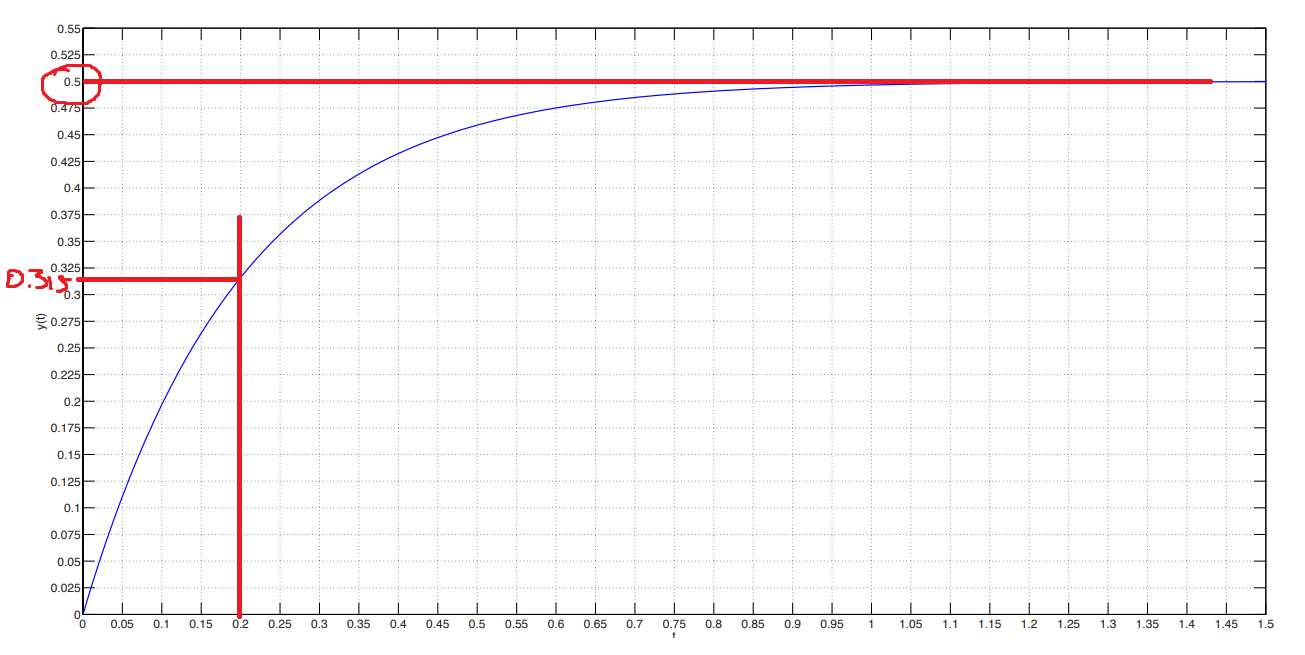
\includegraphics[width=0.9\textwidth]{Questions/Figures/Q1ProblemDiagram.png}
    \caption{System-response to a unit step input with annotations}
    \label{fig:Q1ProblemDiagram}
\end{figure}

\subsection{}
Find the values of the DC gain and time constant of this system \\

\textbf{Solution}\\
The form of a first-order system transfer function is:
\begin{align*}
    G(s) &= \frac{\alpha}{\tau s + 1}
\end{align*}

The DC gain is the value of $y$ as $t \rightarrow \infty$. From the graph, we see that the DC gain is
\begin{empheq}[box=\fbox]{align*}
    G(0) &= 0.5 \\
    \implies \alpha &= 0.5
\end{empheq}

The time constant is the time it takes for the system to reach 63.2\% of its final value. 
\begin{align*}
    y(\tau) &= 0.632 \cdot 0.5 \\
    \implies y(\tau) &= 0.316
\end{align*}

From the graph, 
\begin{align*}
    \boxed{\tau = 0.2}
\end{align*}

\subsection{}
Give the transfer function G(s) of this system\\

\textbf{Solution}\\
Since $\alpha = 0.5$ and $\tau = 0.2$,
\begin{empheq}[box=\fbox]{align*}
    G(s) &= \frac{0.5}{0.2 s + 1}
\end{empheq}